\chapter{Introduction}\label{chapter:introduction}

\section{Motivation}
In recent years,the Internet of Things (IoT) has gathered significant traction which has led to the exponential increase in the number of devices connected to the internet. According to a report released by Cisco \cite{dave}, it is estimated that a total of 50 million devices will be connected to the internet by the year 2020. Data is generated in an enormous amount in real-time by sensors and actuators contained in these devices. With the vast amounts of connected heterogeneous devices,
security and privacy risks are increased. Rapid7 \cite{rapid7}, an  internet security and analytics organization, released a report highlighting vulnerabilities that exist on select IoT devices. In their report, they outline  vulnerabilities in
baby monitors which allowed intruders unauthorized access to devices
whereby a malicious intruder can view live feeds from a remote location. With provenance information, we can generate an activity trail which can be further analyzed to determine who, where, and how, a malicious attack occurred in order to provide preventive measures to eradicate future or current attacks. \cite{cheney_provenance_2009}. 
\par In an IoT system, most of the interconnected heterogeneous devices (things) are embedded systems which
require lightweight and efficient solutions as compared to general purpose
systems. This requirement is attributed to the constrained memory and computing power of such
devices. The vast amount of data generated from IoT
devices requires stronger levels of trust which can be achieved through data
provenance. Provenance is used to determine causality and effect of 
operations performed on data objects \cite{glavic_case_2011}. Data provenance ensures
authenticity, integrity and transparency between information disseminated across an
IoT system. This level of transparency can be translated to various levels across the IoT architectural stack. To achieve transparency in an IoT framework, it is imperative that data provenance and IoT systems be unified to create a provenance aware system that provides detailed records of all data
transactions performed on devices connected in an IoT network. 


Most provenance-aware systems collect a fixed kind of provenance data (e.g system calls, files, and process)  \cite{King:2003:BI:945445.945467, altintas,glavic_case_2011}. There is a need to create provenance-aware systems which allows for the flexibility in specifying the kinds of provenance data to collect. Collecting fixed kinds of provenance leads to  an increase in the amount of noisy provenance data (i.e. unrelated provenance data which is not required by an organization). By doing this, we provide pruning capabilities \cite{braun2006issues} of provenance data. Policy specification and implementation details are discussed in chapter 4.  










\section{Provenance-Aware IoT Device Use Case}

\begin{figure}[tb]
\begin{center}
%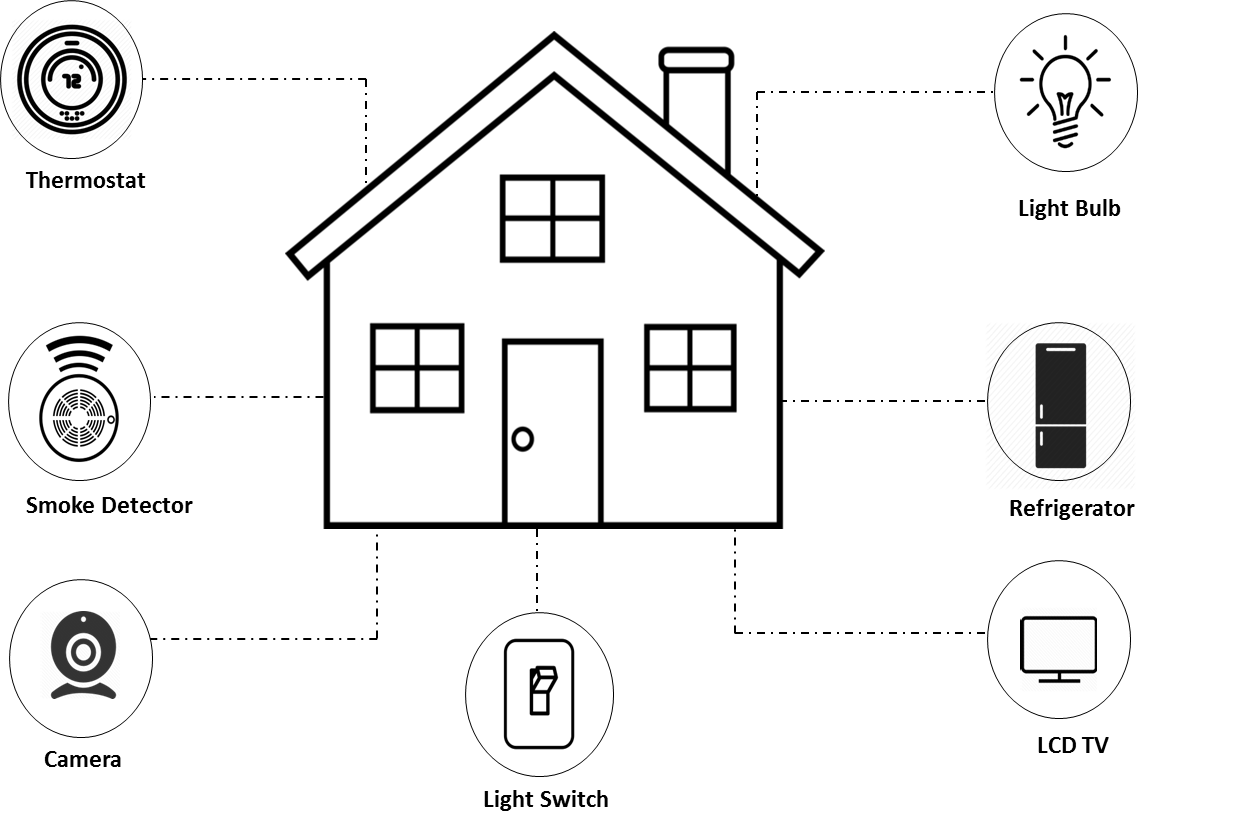
\includegraphics[height=3in]{smart_home_use_case.png}
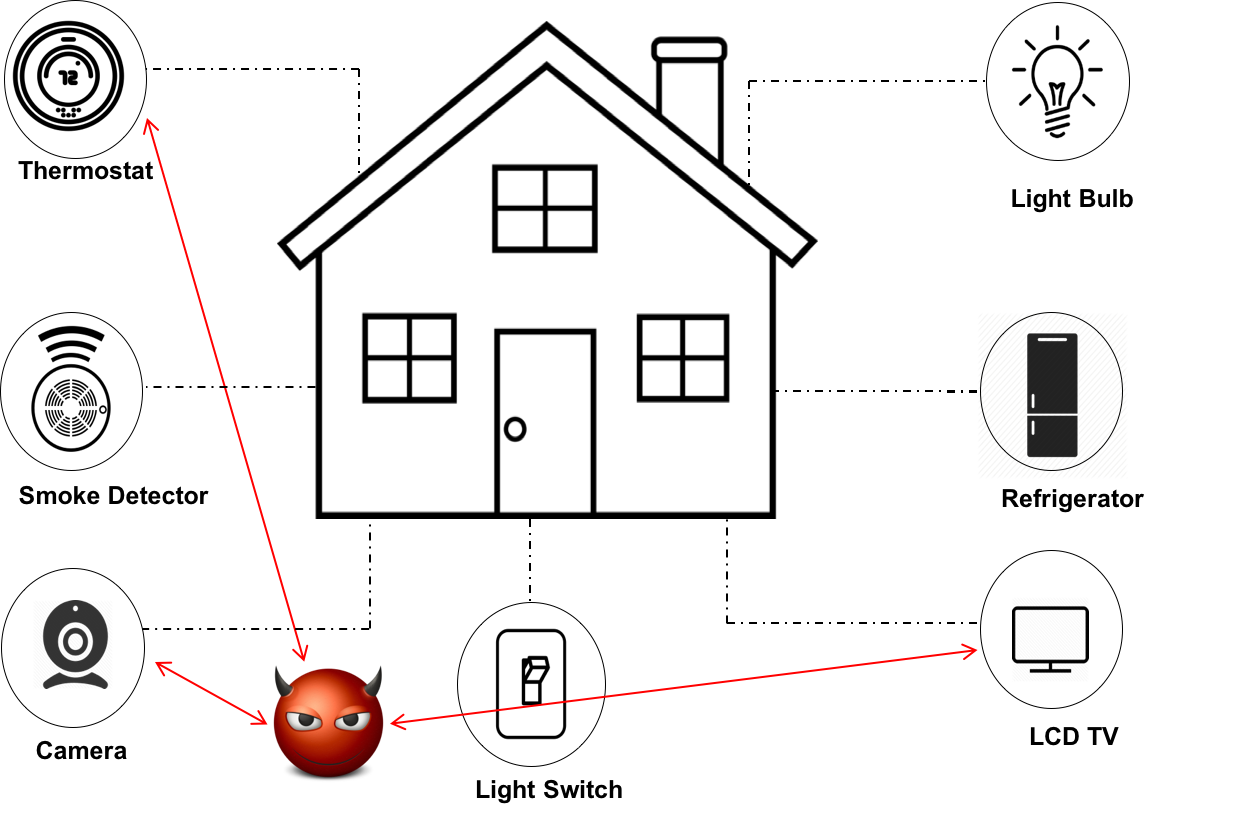
\includegraphics[height=4in]{smart_home_2.png}
\end{center}
\caption{Smart home use case Diagram}
\label{smart_home}
\end{figure}



Consider a smart home as illustrated in Figure \ref{smart_home} that contains interconnected devices such as a thermostat which automatically detects and regulates the temperature of a room based on prior information of a user's temperature preferences, a smart lock system that can be controlled remotely and informs a user via short messaging when the door has been opened or is closed, a home security camera monitoring system, a smart fridge which sends a reminder when food products are low. In an event that a malicious intruder attempts  to gain access to the smart lock system and security camera remotely, provenance information can be used to track the series  of events to determine where and how a malicious attack originated. Provenance can also be used as a safeguard to alert of a possible remote or insider compromise thereby protecting against future or ongoing malicious attacks. 





\section{Research Questions}
The unification of data provenance and IoT is essential to the security of data disseminated in an IoT system. However, the unification raises some important research issues some of which are as a result of pre-existing provenance and IoT related issues. Some of the issues raised as a result of the unification of data provenance with IoT are outlined below:

\begin{itemize}

\item \textbf{Modeling provenance data:} How do we model provenance data collected from sensors and actuators contained in IoT architecture? Are there models used to represent causality between sensor and actuator readings in the IoT architecture.

\item \textbf{Memory constraints on IoT Devices:} The vast amounts of data generated leads to high storage space utilization. Memory and data management techniques should be employed for efficient storage of provenance data on memory constrained devices. How do we effectively collect provenance data in resource constrained devices and relate this information across layers of the IoT architecture



\item \textbf{Provenance data application utilization:} How do we utilize provenance data generated by provenance collection system to provide intrusion detection or digital forensics.



\end{itemize}

\section{Research Contribution}

This dissertation explores the integration of data provenance the IoT ecosystem by making the following key contributions:

\begin{itemize}
  \item \textbf{Provenance-Aware Framework for IoT Device.} A provenance collection framework is important for detecting malicious intrusion by depicting causality and data dependency between entities contained in an IoT ecosystem. By depicting data causality and data dependency,we are able to track changes in information flow of sensor events.This system creates groundwork for capturing and storing provenance data  across the IoT architectural stack.
  
  \item\textbf{Efficient provenance storage using graph summarization.} Prior work has shown that provenance collection frameworks generate immense amounts of provenance data which sometime outgrows data in which provenance is generated for. To address this challenge, an efficient provenance storage approach on IoT devices is developed using graph summarization. 
  
  \item \textbf{Evaluating provenance-aware system using graph based intrusion detection.} Evaluation of provenance collection framework is performed by developing an intrusion detection system which heavily relies on provenance data generated by the provenance collection framework. Evaluation is performed on the graph based intrusion detection system using simulated IoT application: One is a simulated heating air conditioning and ventilation (HVAC) application. \textcolor{red}{The other is an automotive network dataset.}
\end{itemize}

\section{Organization of Dissertation}

The remaining portion of this dissertation is organized as follows: Chapter 2 reviews background information on data provenance and the Internet of Things. It also discusses data provenance model (PROV-DM) for representing provenance. Chapter 3  outlines related work on provenance collection systems. Chapter 4 proposes a provenance collection system for automatic collection of provenance data in an IoT device. It also discusses provenance-sensor model, provenance collection framework's system implementation and evaluation. Chapter 5 describes our framework for efficient provenance storage of provenance data using graph summarization. Chapter 6 concludes with proposed future research directions.

